% Copyright 2009 by Tomasz Mazur
%
% This file may be distributed and/or modified in all ways.


\documentclass[xcolor=pdftex,t,11pt]{beamer}

%%%%%%%%%%%%%%%%%%%%%%%%%%%%%%%%%%
%       SET OPTIONS BELOW        %
%%%%%%%%%%%%%%%%%%%%%%%%%%%%%%%%%%

\usetheme[
% Toggle showing page counter
pagecounter=true,
%
% String to be used between the current page and the
% total page count, e.g. of, /, from, etc.
pageofpages=of,
%
% Defines the shape of bullet points. Available options: circle, square
bullet=circle,
%
% Show a line below the frame title. 
titleline=true,
%
% Set the style of the title page (true for fancy, false for standard)
alternativetitlepage=true,
%
% Institution logo for fancy title page.
% Comment out to remove the logo from the title page.
% IMPORTANT: THERE IS A BUG IN SOME VERSIONS OF PDFLATEX AND FONTS
% ON THE LOGOS ARE NOT RENDERED PROPERLY. IN SUCH A CASE ADD `2` 
% TO THE NAME OF THE LOGO, E.G. comlab2 INSTEAD OF comlab
%titlepagelogo=images/titlepage/ou,
%
% Department footer logo for fancy title page
% Comment out to remove the logo from the footer of the title page/
% IMPORTANT: THERE IS A BUG IN SOME VERSIONS OF PDFLATEX AND FONTS
% ON THE LOGOS ARE NOT RENDERED PROPERLY. IN SUCH A CASE ADD `2` 
% TO THE NAME OF THE LOGO, E.G. comlab2 INSTEAD OF comlab
%titlepagefooterlogo=images/titlepage/comlab,
%
% Institution/department logo for ordinary slides
% Comment this line out to remove the logo from all the pages.
% Available logos are: ou, comlab, comlabinline, comlabou
% IMPORTANT: THERE IS A BUG IN SOME VERSIONS OF PDFLATEX AND FONTS
% ON THE LOGOS ARE NOT RENDERED PROPERLY. IN SUCH A CASE ADD `2` 
% TO THE NAME OF THE LOGO, E.G. comlab2 INSTEAD OF comlab
%ordinarypageslogo=TU-Signet,
%
%
% Add watermark in the bottom right corner
%watermark=<filename>,
%
% Set the height of the watermark.
%watermarkheight=100pt,
%
% The watermark image is 4 times bigger than watermarkheight.
%watermarkheightmult=4,
]{Torino}

% Select color theme. Available options are:
% mininmal, greenandblue, blue, red
\usecolortheme{blue}

%Select different font themes.Available options are:
% default, serif, structurebold, structureitalicserif, structuresmallcapsserif
\usefonttheme{structurebold}

\usepackage{tikz}
\usepackage{pgf}

\pgfdeclareimage[height=6ex]{ou-logo}{images/ou}

\logo{\pgfuseimage{ou-logo}}

\usepackage{listings}

\lstset{language=C,
 basicstyle=\tiny
 }

\usepackage{ifthen}

\usepackage{moreverb}
\usepackage{pgf}
\usepackage{tikz}
\usetikzlibrary{arrows, automata, shapes.multipart, chains, positioning, fit}

\usepackage{pifont}
\newcommand{\xmark}{\ding{55}}

\usepackage{color}
\definecolor{light-gray}{gray}{0.80}

\lstset{escapeinside={<@}{@>}}


%%%%%%%%%%%%%%%%%%%%%%%%%%%%%%%%%%
%       PRESENTATION INFO        %
%%%%%%%%%%%%%%%%%%%%%%%%%%%%%%%%%%

\author{Cristina David \and Daniel Kroening \and Matt Lewis}
\title{Unrestricted Termination and Non-Termination Arguments for Bit-Vector Programs}
%\subtitle{}
\institute{Oxford University}
\date{\today}

\begin{document}



%%%%%%%%%%%%%%%%%%%%%%%%%%%%%%%%%%
%       SLIDE DEFINITIONS        %
%%%%%%%%%%%%%%%%%%%%%%%%%%%%%%%%%%

\begin{frame}[plain]
  \titlepage
\end{frame}

\begin{frame}{Outline}
  \tableofcontents
\end{frame}

\section{What's The Problem?}
\begin{frame}[fragile]{Motivation}
Does this program terminate?
\begin{center}
\begin{minipage}{0.4\linewidth}
 \begin{lstlisting}[language=C,basicstyle=\normalsize]
while (x > 0) {
  x++;
}
 \end{lstlisting}
\end{minipage}
\end{center}

\pause

That depends...

It \emph{does not} terminate if the program operates on integers...

But it \emph{does} terminate if the program operates on fixed-width words
(-x decreases monotonically and is bounded by -MAXINT).

\end{frame}

\begin{frame}[fragile]{Motivation}
Which of these guys terminates?
\begin{center}
\begin{minipage}{0.45\linewidth}
 \begin{lstlisting}[language=C,basicstyle=\normalsize]
while (x > 0) {
  x = (x - 1) & x;
}
\end{lstlisting}
\end{minipage}
\begin{minipage}{0.45\linewidth}
 \begin{lstlisting}[language=C,basicstyle=\normalsize]
while (x > 0) {
  x = (x + 1) & x;
}
\end{lstlisting}
\end{minipage}
\end{center}

\pause

The left one does (x decreases monotonically), but the right one doesn't ($2 \rightarrow 2 \rightarrow \dots$).
\end{frame}

\begin{frame}{Motivation}
Proving program termination has been a big deal for a while.

\vspace{1em}

It's still quite hard to do for the programs that people write, which use bitvectors and all kinds of nonsense.
\end{frame}


\subsection{Termination Is Hard}


\subsection{Bitvectors Are Hard}

\begin{frame}[fragile]{Bitvector Termination}
 \begin{columns}[c]
  \column{.45\textwidth}
  \emph{If a program terminates for integers, it terminates for bitvectors.}

  \uncover<2->{{\centering \color{red} \Huge \xmark
  
  }
  
  \lstinputlisting[language=C,basicstyle=\normalsize,mathescape]{term1.c}
  }

  \column{.45\textwidth}
  \emph{If a program terminates for bitvectors, it terminates for integers.}

  \uncover<3->{{\centering \color{red} \Huge \xmark
  
  }
  
  \lstinputlisting[language=C,basicstyle=\normalsize]{term2.c}
  }
 \end{columns}

 \vspace{1.5em}
 
 \uncover<4->{\Large \centering Integer and bitvector termination are incomparable!
 
 }
 
\end{frame}


\begin{frame}{Bitvector Termination}
\begin{quote}
 ``People really don't *think* about termination using bitvector arguments''
   \hspace*\fill{\small--- Anonymous}
\end{quote}
\end{frame}


\subsection{Non-Linearity Is Hard}



\begin{frame}{Example}
\end{frame}

\section{Our Solution}

\subsection{Existential Second-Order Logic}

\begin{frame}[fragile]{Our Theory}
 We will try to build termination proofs by solving \emph{second-order constraints}.

 \vspace{1em}

 Specifically, we will build constraints of the form:

 \begin{center}
 \begin{columns}
  \column{.15\textwidth}
  $\exists {\textcolor{red} F} . \forall \vec{\textcolor{blue} x} . {\textcolor{green} \phi}({\textcolor{red} F}, \vec{\textcolor{blue} x})$

  \column{.4\textwidth}
  \begin{minipage}{\textwidth}
 \begin{itemize}
  \item[$\textcolor{red} F$] a function.
  \item[$\textcolor{green} \phi$] a quantifier free formula.
  \item[$\vec{\textcolor{blue} x}$] the program variables.
 \end{itemize}
 \end{minipage}
 \end{columns}

 \end{center}

 \vspace{.75em}

 These constraints can be solved using an EPR solver (such as the one in Z3), or by using a program
 synthesiser to synthesise $\textcolor{red} F$.
\end{frame}


\begin{frame}[fragile]{Modelling Loops}
 For ease of presentation, we will consider loops of the following form:

 \begin{center}
 \begin{columns}[c]
  \column{.15\textwidth}
  \begin{minipage}{\linewidth}
 \begin{lstlisting}[language=C,basicstyle=\normalsize]
<@\textcolor{red}{P}@>;

while (<@\textcolor{green}{G}@>) {
  <@\textcolor{blue}{B}@>;
}
 \end{lstlisting}
 \end{minipage}
 
 \column{.4\textwidth}

 \begin{minipage}{\linewidth}
 \begin{itemize}
  \item[\textcolor{red}{P}] the prefix to the loop.
  \item[\textcolor{green}{G}] the loop guard.
  \item[\textcolor{blue}{B}] the loop body.
 \end{itemize}
 \end{minipage}
 \end{columns}

 \end{center}

 
\end{frame}


\subsection{Ranking Functions: Proofs of Termination}

\subsection{Recurrent Sets: Proofs of Non-Termination}
\subsection{Using Tautologies}

\section{Experiments}

\begin{frame}[fragile]{Fin}

\begin{center}
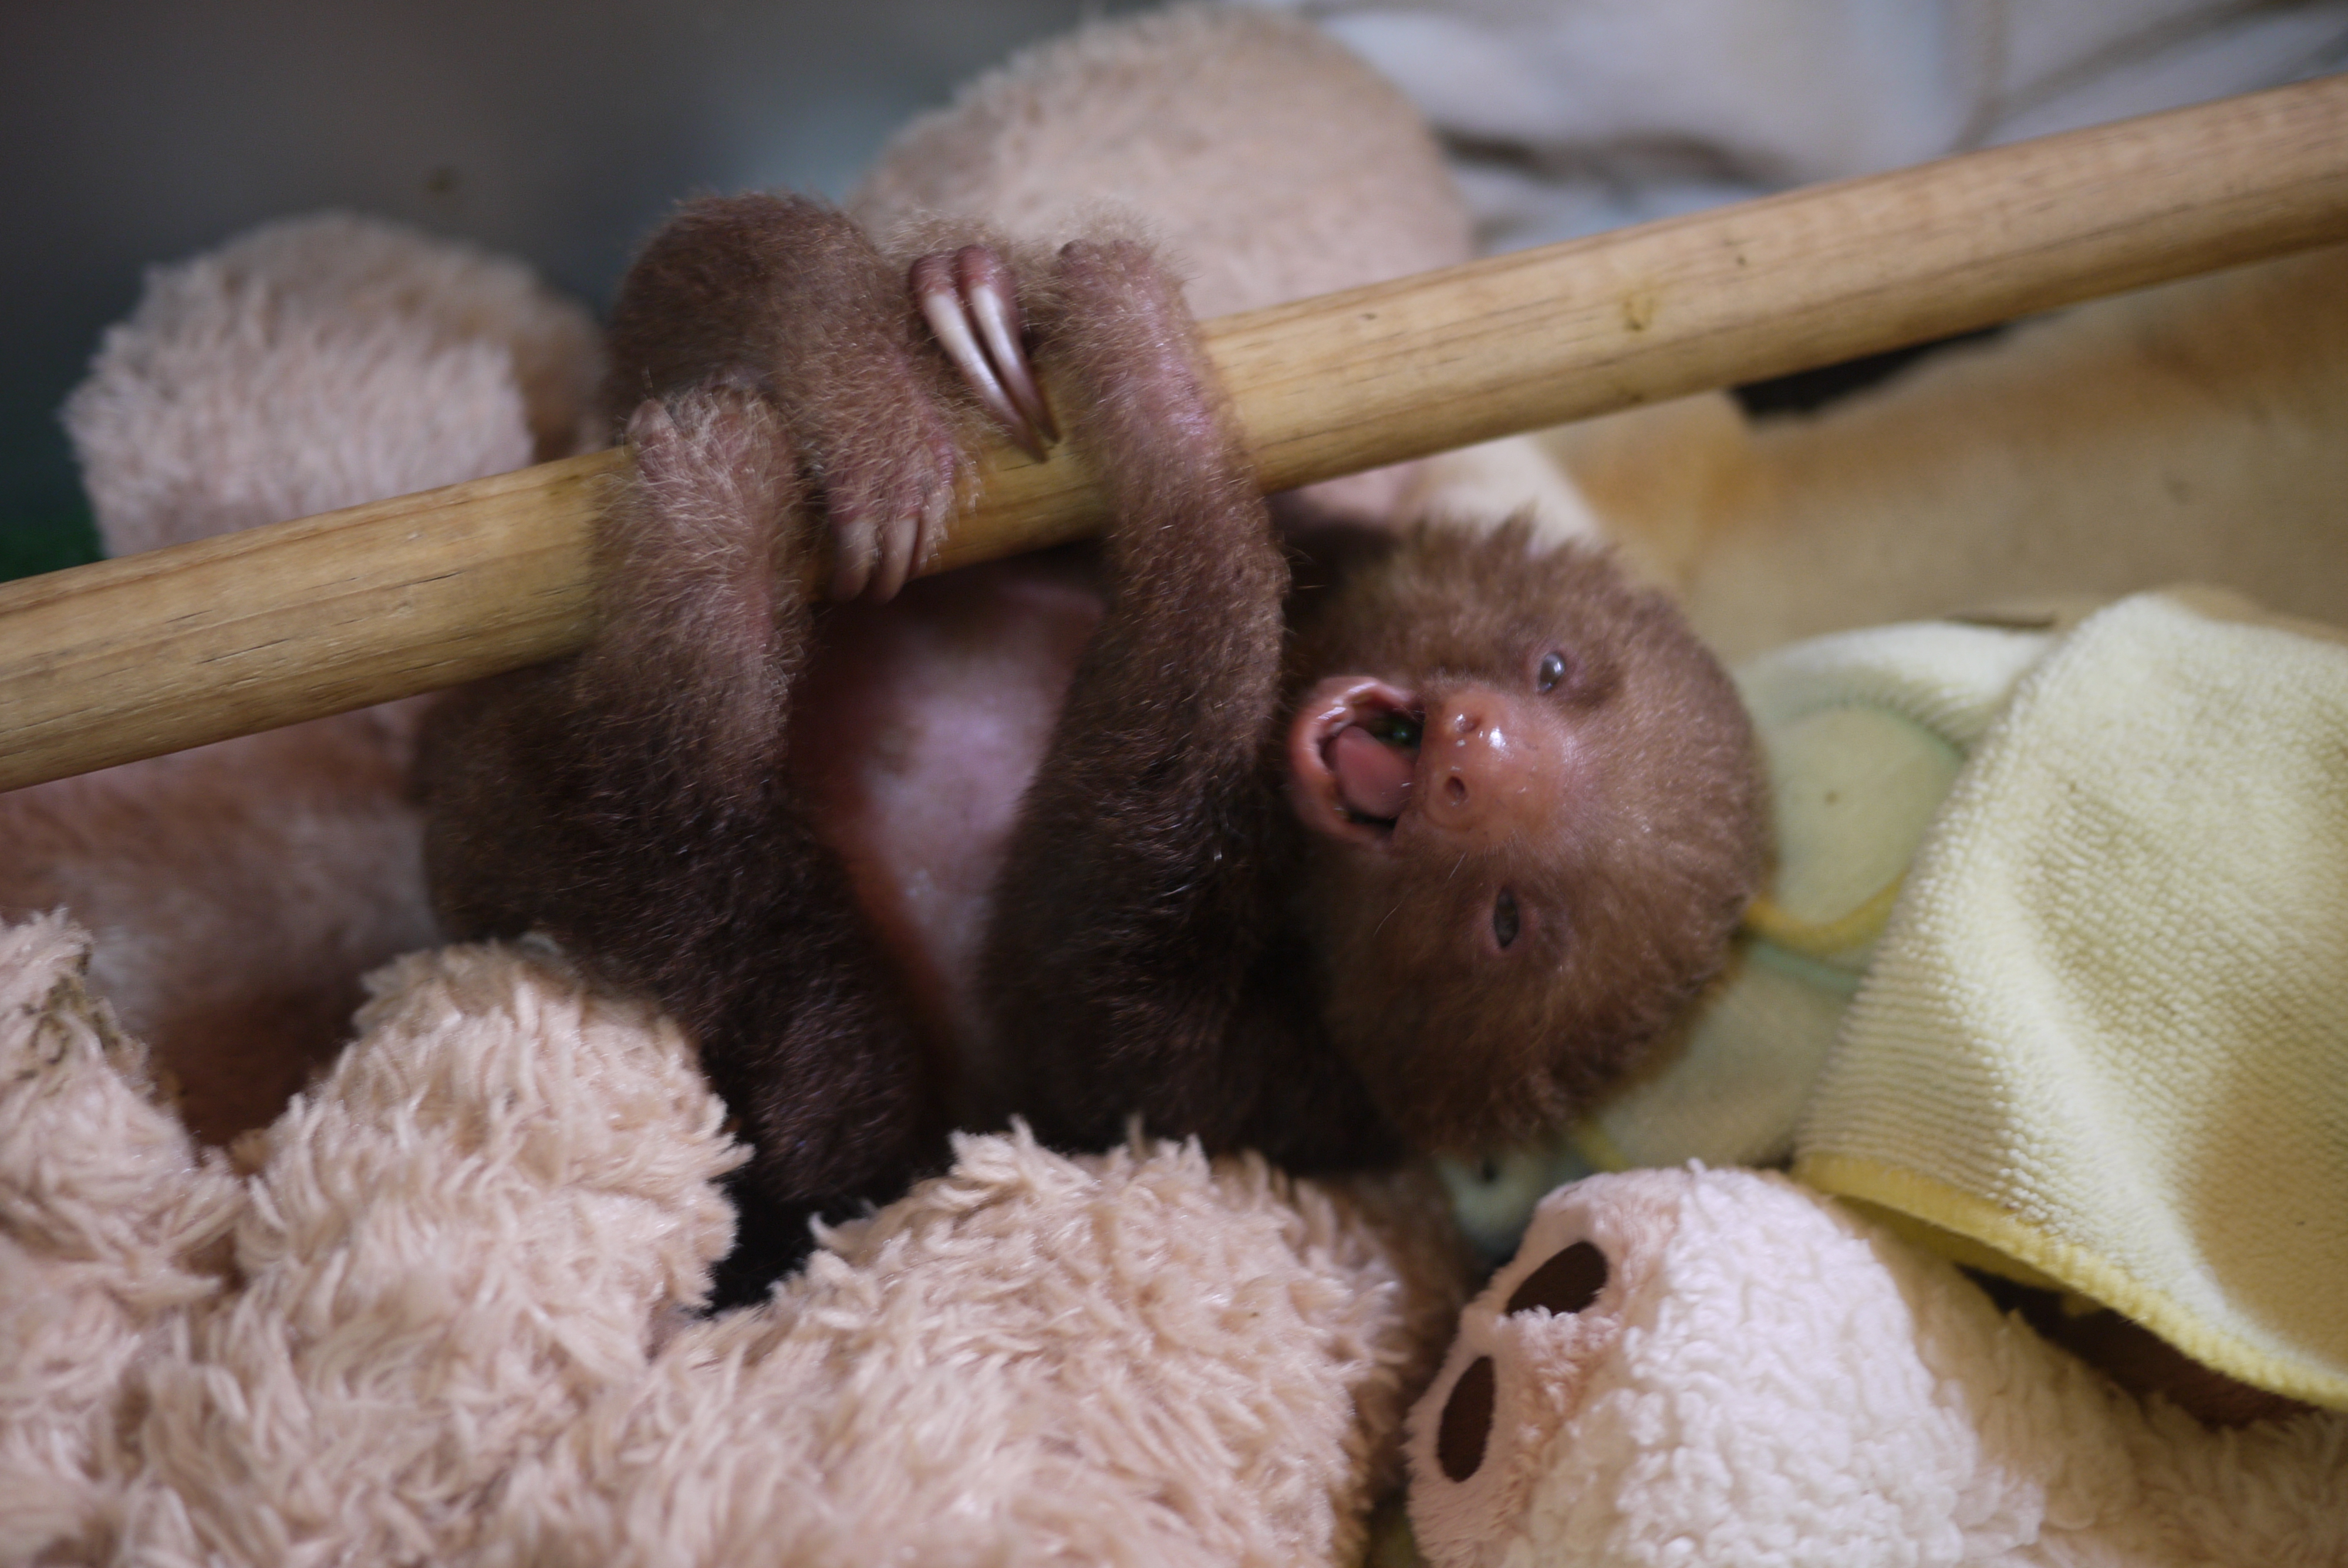
\includegraphics[width=.7\textwidth]{sloth.jpg}

\Huge
 Thank you!
\end{center}

\end{frame}


\end{document}
